\chapter[Data Discovery Systems for Planetary Science]{Data Discovery Systems for Planetary Science}
\label{ch:msl}
This chapter is from my published work \cite{horton2021integrating} and is included here as the groundwork for the novelty detection systems I go on to use in Chapters \ref{ch:spectra} and \ref{ch:rst}.
Being one of the first projects I undertook in my research career, this chapter describes the steps taken to operationalize novelty detection methods for use in planetary science for the Mars Science Laboratory (MSL) Curiosity rover.
This chapter focuses on how to take theoretical novelty detection methods and create a pipeline to integrate them into the tactical planning process for MSL.
In addition to the original publication, this chapter has been updated to include work conducted on the Planetary Data System (PDS) Image Atlas to provide new methods for users to search for information \cite{horton2020novelty}.
This chapter is included in this dissertation to provide a foundational understanding of how novelty detection systems can be operationalized.
By detailing the integration of this system into the Mars Science Laboratory (MSL) tactical planning pipeline, the practical challenges and solutions involved in adapting machine learning techniques for real-world scientific missions are highlighted.
The insights gained from this work serve as a basis for the on-board novelty detection methods developed to support mission operations for missions such as ASTHROS and RST. 

\section{Abstract}
While innovations in scientific instrumentation have pushed the boundaries of Mars rover mission capabilities, the increase in data complexity has pressured Mars Science Laboratory (MSL) and future Mars rover operations staff to quickly analyze complex data sets to meet progressively shorter tactical and strategic planning timelines. 
MSLWEB is an internal data tracking tool used by operations staff to perform first-pass analysis on MSL image sequences, a series of products taken by the Mast Camera, Mastcam. 
Mastcam consists of a pair of 400-1000 nm wavelength cameras on MSL's Remote Sensing Mast that, among other functions, uses a filter wheel to produce multispectral images by creating a sequence of products at different wavelengths. 
Mastcam's multiband multispectral image sequences require more complex analysis compared to standard 3-band RGB images. 
Typically, these are analyzed by the inspection of false color images created to aid visualization, such as band ratios between different spectral indices that can highlight specific potential mineralogic differences among iron-bearing phases and decorrelation stretches to enhance the color differences between multiple filters. 

Given the short time frame of tactical planning in which downlinked images might need to be analyzed (within 5-10 hours before the next uplink), there exists a need to triage analysis time to focus on the most important sequences and parts of a sequence. 
We address this need by creating products for MSLWEB that use novelty detection to help operations staff identify unusual data that might be diagnostic of new or atypical compositions or mineralogies detected within an imaging scene. 
This was achieved in two ways: by creating products for each sequence to identify novel regions in the image and by assigning multispectral sequences a sortable novelty score. 
These new products provide colorized heat maps of inferred novelty that operations staff can use to rapidly review downlinked data and focus their efforts on analyzing potentially new kinds of diagnostic multispectral signatures. 
This approach has the potential to guide scientists to new discoveries by quickly drawing their attention to often subtle variations not detectable with simple color composites.
The products developed in this work have shown promising benefits for integration into mission operations by potentially decreasing tactical operations planning time through guided triage.

\section{Introduction}
While discovering the unexpected is one of the most exciting parts of research, the process of making a discovery often involves countless hours of sifting through otherwise mundane data. 
Advances in novelty detection systems can help to alleviate this arduous task by enabling researchers to focus their attention on the most interesting parts of their data. 
Novelty is defined as an unexpected occurrence in a sequence based on a data set of typical sequences.
Given what is known to be "normal," the novelty detection algorithm highlights the most unusual features in an image. 
Novelty detection techniques work by analyzing the commonalities in a data set in order to generalize the structure of the data and pick out anomalies \parencite{japkowicz1995novelty}.
When a new observation is presented to a novelty detection system, the system identifies features that differ from the commonalities learned during training \parencite{markou2003novelty}.
This is different from traditional classification systems as what constitutes as \textit{novel} is not predefined. 
Instead of classifying samples as \textit{typical} and \textit{novel}, novelty detection systems build a model from \textit{typical} examples that can be used to discover anomalies. 
This makes novelty detection ideal for scenarios where \textit{novel} examples are infrequent or difficult to obtain and \textit{typical} examples are abundant \parencite{japkowicz1995novelty}.
Identifying anomalous examples is useful in many application domains, such as structural fault detection for aerospace systems by analyzing ambient vibrations \parencite{worden1997structural} or identifying brain tumors using MRI images \parencite{wang2020brain}.

\begin{figure}
\centering
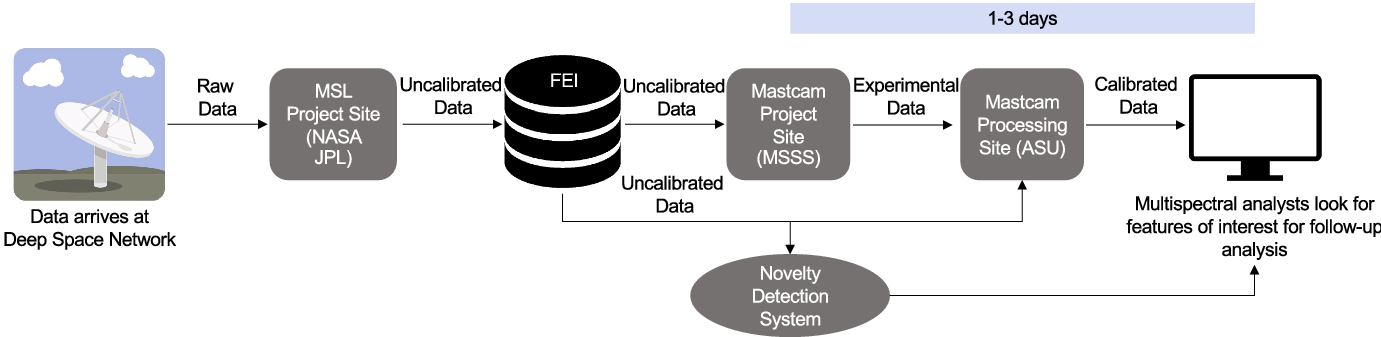
\includegraphics[width=\linewidth]{figs/msl/DSN.png}
\caption[Mastcam Image Processing Pipeline]{Illustration of the Mastcam image processing pipeline \protect\parencite{kerner2020comparison}}
\label{msl/fig:timeline}
\end{figure}

Planetary science is another domain where novelty detection proves useful. 
Due to the rapid turn-around required for tactical planning for landed Mars missions, efficient data analysis methods need to be employed to analyze data from scientific instruments \parencite{bell2019tactical}.
With high volumes of downlinked data, tactical operations planning teams have to quickly perform ground analysis to meet the ten-hour turn-around time for MSL operations to uplink commands \parencite{samuels2013preparation}. 
The timeline is even shorter for the upcoming Mars 2020 mission, which has a desired five-hour turn-around time \parencite{wilson2017nasa}.
During tactical planning, the MSL Curiosity rover sends compressed observations through one of three Mars orbiters to the Deep Space Network (DSN) on Earth so that operations team members can use these observations to make plans for the next sol \parencite{kerner_multispec}.
Rapid analysis is required for tactical planning as discoveries made outside of the time frame are subject to increased mission resource cost as the rover may need to reverse course to re-visit the target \parencite{kerner2020comparison}.
This need for rapid analysis makes systems that can quickly extract information and identify regions of interest in scientific data vital to efficient tactical planning. 

Additionally, on the ground, data from missions like MSL are often observed by both scientists and the public.
The Planetary Data System (PDS) Image Atlas is a tool for both scientists and enthusiasts to explore vast image sets from various planetary missions. 
Like a good photographer, some mission instruments take multiple views of the same scene in order to best capture a subject. 
When browsing an instrument's reverse chronological photo album, an Image Atlas user may encounter large batches of nearly identical images. 
This experience is not user-friendly for both scientists, who may be looking for specific types of images, and enthusiasts, who may just be browsing a mission. 
To assist in navigation, the Image Atlas offers tools to filter and classify images by metadata, including time of collection, instrument used, and content (e.g., craters, dunes, layered rocks) \cite{wagstaff2018deep}.
These navigation techniques work for users researching specific interests but are less useful for users looking to browse the image set. 
To find interesting or unique examples, users must manually browse through the Atlas, which can be a time-consuming and impractical process.

This work primarily focuses on the Mastcam imaging system on the MSL Curiosity rover.
Mastcam consists of a pair of multispectral Charge Coupled Device (CCD) imagers on MSL that are each capable of using an eight-position filter wheel to take red, green, and blue (RGB) images as well as multispectral images in nine bands from 400 to 1100 nm (visible to near-infrared) \parencite{bell_mastcam}.
A set of image products from Mastcam is called a sequence.
Seven of the eight landed missions on Mars have employed camera systems capable of multispectral imaging \parencite{bell2019tactical}.
Future missions, such as Mars 2020 and Psyche, will also be carrying similar multispectral cameras \parencite{bell2016mastcam} \parencite{bell_psyche}.
Given that multispectral cameras are so prevalent in planetary exploration, the ability to rapidly detect novel features in multispectral images is beneficial across many missions.

The goal of this work is to operationalize previous work developed for novelty detection for Mastcam.
\cite{kerner2020comparison} quantitatively compared different novelty detection methods for the analysis of multispectral images on Mars.
With a typical data set, machine learning models including Reed-Xiaoli (RX) detectors, Principal Component Analysis (PCA), Generative Adversarial Networks (GANs), and Convolutional Autoencoders (CAE) were used to produce a measure of how atypical each image or multispectral pixel is in a new sequence. 
Using pixel-wise analysis allows these methods to highlight difficult to identify novel regions within an image that may otherwise go undetected by operations staff.
These methods\footnote{https://github.com/JPLMLIA/mastcam-noveltydet} and the data set\footnote{https://zenodo.org/record/3732485} used to evaluate them were made publicly available at publication. 
Multiple models were evaluated to show that certain models perform better for certain novelties than others: e.g., PCA was better suited for detecting spectral (compositional) novelties than for morphological (shape) novelties. 
Their work provides an in-depth qualitative evaluation of these methods, which was used to guide decisions about which methods to use. 
While their work demonstrated the capabilities of the algorithms, it did not evaluate the methods based on their effectiveness in the tactical planning pipeline.
In order to be most useful to operations, these methods need to be automatically run on new data and integrated into tactical analysis workflows to accelerate tactical planning \parencite{donahoe2020new}.
New advances in this work include further development of the algorithms and the creation of an implementation strategy for operations. 
Additionally, we analyzed the outputs from the system to determine the usefulness of these methods in comparison to existing tactical planning procedures. 

As an example of how these methods can be used, we created a pipeline to integrate novelty detection into the PDS Image Atlas.
To meet users' needs, we implemented several image novelty and discovery tools.
These tools can be used by the Image Atlas to display images for users looking to browse an image set in a more relevant manner. 
The novelty tools are used to show users the most interesting examples in an image set, and the discovery tools are used to show a diverse set of examples in an image set.

\section{Related Work}
Novelty detection is a form of anomaly detection that focuses on detecting novel examples in a data set \parencite{domingues2019comparative}. 
Given what is known to be typical in a data set, these algorithms find novel examples that may be unknown to the user.
Unlike a classifier, novelty detection systems detect whether an input is similar to examples in the typical training set or if the input is novel \parencite{markou2003novelty}.
Novelty detection can be seen as a one-class classification task where a model is trained to describe a data set of typical examples \parencite{pimentel2014review}. 
For novelty detection, the training data represent a set of examples that an end user would identify as typical examples. 
When the model is used to infer the novelty of new data, the system calculates how different the new examples are compared to the training set. 
As abnormal examples are not well represented in the training set, novelty detection systems are not able to model abnormalities and thus highlight them as novel. 
This allows novelty detection systems to highlight abnormal data by evaluating how well (or how poorly) they can model the examples. 
These methods can be applied to various domains such as fraud detection based on card activity \parencite{oosterlinck2020one}, human verification for websites from mouse and keyboard usage \parencite{kim2018keystroke}, fault detection for aerospace systems by analyzing ambient vibrations \parencite{worden1997structural} and brain tumor identification using MRI images \parencite{wang2020brain}.

This work is based on previous work that developed novelty detection for multispectral images on Mars \parencite{kerner2020comparison}.
Figure \ref{msl/fig:timeline} shows the current pipeline for multispectral image processing for operational analysis and where we propose to augment the pipeline with novelty detection systems. 
Calibrated data are often not available during the tight tactical analysis schedule, so uncalibrated data will be used for novelty analysis. 
Current methods for quick analysis involve generating quick look products, such as decorrelation stretches and filter ratios, which help to identify spectral changes in the sequence \parencite{gillespie1986color}.
For example, comparing the relative reflectance spectra of two different drill tailings can inform analysts of the similarities and differences in mineral composition \parencite{wellington2017visible}.
These quick-look products are generated using calibrated data, making them unavailable during the tactical analysis time frame.  

Kerner et al.~demonstrated four types of novelty detection systems for multispectral novelty detection: CAEs, GANs, PCA, and RX detectors \parencite{kerner2020comparison}. 
All of these methods, except RX, are reconstruction-based methods that attempt to "compress" and "reconstruct" an input to recreate the original image. 
When trained on typical examples, these methods are able to reconstruct normal examples well but are unable to represent novel examples.
The novelty detection system is able to identify novel regions based on the reconstruction error, which is the difference between the input and the recreated image.
For Mastcam multispectral sequences, these images have six bands instead of the traditional one (grayscale) or three (RGB). 
It is important to note that Kerner et al.~evaluated these methods to identify novel geology in multispectral sequences, not create a visualization for tactical analysis that maximizes their ability to spot hard-to-find features. 
Our goal is to create novelty detection products that could be integrated into actual tactical operations pipelines and evaluate their effectiveness for triaging analyst time in tactical operations.

\section{Data Set}
%%%%%%%%%%%%%%%%%%%%%%%%%%%%%%%%%%%%%%
\begin{figure*}
\centering
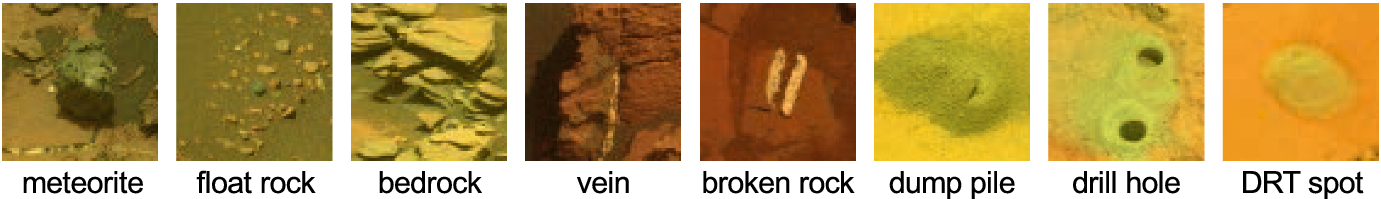
\includegraphics[width=\linewidth]{figs/msl/categories.png}
\caption[Novel Geology Categories for Mastcam Multispectral Images]{Examples from the eight categories of novel geology in the Mastcam multispectral image data set \protect\parencite{kerner_data}.}
\label{msl/fig:NovelCategories}
\end{figure*}

In this work, we created a data set of all multispectral Mastcam sequences based on the preprocessing methods outlined in the labeled Mars multispectral novelty detection data set \parencite{kerner_data}.
This previous data set provided images with both \textit{typical} and \textit{novel} labels cropped from the M-100 right eye of Mastcam on MSL between sols 1 to 1666.
Each example in the data set is a 64-by-64 tile with six bands corresponding to 6 different filters.
The tiles were sub-sampled from larger thumbnail images of around 140-by-100 pixels in size. 
Thumbnails were used rather than full-resolution sequences as they are among the first available products during tactical planning. 
Additionally, uncalibrated images were used as these data are the most readily available in the tactical analysis timeline. 
To generate the data set, these thumbnails were loaded as single-band images in OpenCV before combining them to produce a single six-band tile \parencite{opencv_library}.

While we did not explicitly use the labeled Mars multispectral novelty detection data set in this work, we utilized the novelty classes to verify the system.
The data set provided a set of novel tiles divided into eight sub-classes: meteorite, float rock, bedrock, vein, broken rock, dump pile, drill hole, and DRT spot, as shown in Figure \ref{msl/fig:NovelCategories}. 
Multispectral analysts from the Mastcam operations team identified novel geology in images using bounding boxes based on operations experience and past publications of high-interest targets (e.g., \cite{wellington2017visible}).
Sub-sampled tiles that intersected with these bounding boxes were included in the novel data set.

The goal of this work is to triage tactical analysis time by prioritizing interesting images and highlighting features that are otherwise difficult to identify in multispectral sequences.
While our system should be able to identify novelties such as large veins and broken rocks, which are relatively easy for analysts to identify in RGB or single-band images, highlighting these examples will not reduce tactical analysis time as much as other features that are difficult or impossible to see without detailed analysis of multispectral sequences. 
%they can be easily seen without a novelty detection system.
%Many of the examples in the original training set contain novelties that a tactical operations staff member could easily spot. 
%These examples are visible in the RGB images and do not require a novelty detection system to draw attention to them.
The \cite{kerner2020comparison} data set did not account for these operational priorities when evaluating novelty detection performance. 
In order to fully evaluate the benefit of our novelty detection system in tactical operations, we created a new data set using the same preprocesssing as the Kerner et al. data set. 
Instead of separating the images into typical and novel data sets, we included all multispectral sequences from Mastcam's left and right eyes in an unsupervised manner.
The images in this data set were preprocesssed in the same way as the original data set but kept as full-size thumbnails instead of tiles in order to provide detections at the same resolution as they are viewed by operations staff. 
Starting with every thumbnail taken by Mastcam, the data set was filtered by sequences containing seven different filters: RGB (no filter) and six narrow-band spectral filters.
Additionally, sequences containing the calibration tool were omitted. 
This filtering resulted in about 900 total sequences split between the left and right eye. 
The six narrow-band sequences were used as inputs into the algorithm, and the RGB was used for reference.
%%%%%%%%%%%%%%%%%%%%%%%%%%%%%%%%%%%%%%
\section{Methods}
%%%%%%%%%%%%%%%%%%%%%%%%%%%%%%%%%%%%%%
In this work, we employed a pixel-wise RX method for novelty scoring.
Pixel-wise RX is a distribution-based method that calculates the distance between each pixel in a test image and a background distribution, which can be visualized at the image level as a heatmap of novelty scores. 
In comparison with other methods, pixel-wise RX is outperformed when identifying images with certain types of novelties, such as float rocks, veins, bedrock, and broken rock, but performs better for other novel categories. 
While this may seem like RX is a poor choice for novelty detection, the novelty scores in \cite{kerner2020comparison} were aggregated to image-level scores and did not compare algorithms on the basis of their ability to highlight novel pixels in an image in a way that is useful for tactical planners. 
Pixel-wise RX may not have the highest performance for all types of novelty, but its scores and their associated visualizations are relatively simple and interpretable compared to other methods. 
This is an important characteristic in method selection for analysts using novelty detection methods in a tactical operations setting. Thus, we chose to use pixel-wise RX to develop novelty-based tactical planning products. 
%Of the novelty detection methods discussed in previous work, algorithms that are sensitive to spectral novelties are most desirable. 
%Spectral novelties are novelties occurring due to unexpected differences in the spectrum of an object and not from the actual shape of the object.
%Methods to detect structural novelties typically pick out features visible in standard RGB images. 
%As the goal of this system is to identify novelties that are not easily observable in the uncalibrated sequences, finding structural novelties is not necessary. 
%While hard to spot structural novelties do exist, we have chosen to focus on spectral novelties as these tend to be more difficult to spot visually. 

In this study, we chose to focus on spectral novelties that are difficult for analysts to spot because they require analysis across multiple filters to find correlations that are difficult to identify when looking at each image separately. 
%The method chosen to detect spectral novelties is pixel-wise RX as previous work has shown it is best suited for identifying novelties with spectral differences when compared with CAEs, GANs, and PCA \parencite{kerner2020comparison}.
While methods not based on novelty detection exist that help identify spectral novelties, they require calibrated data, which are often unavailable during the tactical time frame. 

Unlike the other algorithms considered, RX is not a reconstruction-based method for detecting novelties.
Instead, RX computes a background distribution from typical examples and compares this distribution to infer the novelty of pixels in new images \parencite{reed1990adaptive}.
For novelty detection in Mastcam sequences, the background is computed using the spectrum from each pixel in all sequences in order to generalize the entirety of the data set. 
For a multispectral image with $n$ filters, the background distribution is defined by the $n \times 1$ mean spectrum vector, $\boldsymbol{\mu}$, and an $n \times n$ covariance matrix, $\boldsymbol{\Sigma}$, of all pixels in the training set \parencite{guo2016anomaly}.
This provides a mean for each multispectral band and a covariance matrix for the band pairings. 
To infer the novelty in a new image, $\boldsymbol{X}$, an RX score is calculated for each $n \times 1$ pixel vector, $\boldsymbol{x}_i \in \boldsymbol{X}$, using the Mahalanobis distance between the background and the filter response values as shown in Equation \ref{msl/eq:RX_eq}.
\begin{equation}
    \label{msl/eq:RX_eq}
    \text{RX}(\boldsymbol{x}_i) = (\boldsymbol{x}_i - \boldsymbol{\mu})^T \boldsymbol{\Sigma}^{-1} (\boldsymbol{x}_i - \boldsymbol{\mu})
\end{equation}
This score will be referred to as the pixel novelty score, as it is a measure of how novel a pixel is relative to the background distribution. 
As this method is pixel-based, the dimension size of the sequence does not matter, so inferences can be run on sequences of any resolution.
This is particularly useful for Mastcam as the height of each sequence of images varies. 

After computing the RX background distribution using typical sequences, Equation \ref{msl/eq:RX_eq} can be applied to new sequences to identify novel features.
Each sequence can be analyzed individually or relative to other sequences based on their pixel novelty scores. 
To reduce the effect of brightness in the novelty scoring, separate models were created using a data set where the RGB image of the sequence is loaded as a grayscale image and used to divide the other six images in the input. 
Individual sequence analysis is accomplished by visualizing the pixel novelty scores as a heat map. 
Analysts can quickly review these heat maps to identify the most novel regions within a sequence relative to all prior sequences. 
Statistics can be calculated and sorted for each sequence to compare the novelty of different sequences.
This can help prioritize which multispectral sequence to review first. 

\subsection{PDS Image Atlas Integration}
To integrate these tools into the Image Atlas, Amazon Web Services (AWS) SageMaker (SM) was used to train and deploy these tools as queryable endpoints. 
SM allows developers to utilize a hosted Jupyter Notebook instance to deploy training jobs and inference endpoints on Elastic Compute Cloud (EC2) instances. 
In most cases, training data is loaded using the PDS Image Atlas API \parencite{grimes2018pds}. 
A training job is deployed to an EC2 instance, and a model is saved in a Simple Storage Service (S3) bucket. 
SM is then used to create an inference endpoint by paring the model in the S3 bucket with an EC2 instance. 
Once the inference endpoint is made, it can be exposed outside of AWS using a Lambda function and the API Gateway.

Image discovery is the process of identifying images of high content diversity in a dataset.
We use an unsupervised novelty detection algorithm, requiring no prior knowledge of the dataset. 
An image dataset is used as input, and the result is N images of diverse content, where N is a value specified by the user. 
An example use case for this is having a carousel of images with high content diversity on the PDS Image Atlas website to give users a sample of a variety of images gathered from a particular mission or instrument.

A pre-trained convolutional neural network (CNN) is used to extract feature vectors from each image in the data set, and then Discovery via Eigenbasis Modeling of Uninteresting Data (DEMUD) is run, which is an algorithm that detects novel items in a dataset \parencite{wagstaff_demud}.
DEMUD selects interesting or novel images in a dataset with an iterative method where an item is selected from the dataset. 
Image content is modeled with a singular value decomposition (SVD). 
The remaining items are projected onto the model, and a reconstruction error is calculated for each item not already included in the SVD model. 
The item with the highest reconstruction error, or the most novel item, is then selected and incorporated into the model. 
This enables the model to learn about the most novel items and avoid selecting them for future iterations. 
This process continues until the N most diverse images are selected. 
%%%%%%%%%%%%%%%%%%%%%%%%%%%%%%%%%%%%%%
\section{Results}
%%%%%%%%%%%%%%%%%%%%%%%%%%%%%%%%%%%%%%
%Using the training set created from all the sequences, a background distribution was created for the typical Mastcam multispectral pixel. 
%This background distribution was used to generate pixel novelty scores for each sequence in this same data set.
To assess the system's performance for the novel features in the \cite{kerner_data} data set, we located the full-size thumbnails of a selection of the novel tiles from each category and verified that the novelties highlighted in the new images were self-consistent with previous results in the tiles. 
The novelty detection system using pixel-wise RX performs well in highlighting easy-to-spot novelties in the data set. 
Figure \ref{msl/fig:easyNovel} shows examples of some of the easy-to-catch novelties that the system is able to detect. 
We claim that these examples are relatively easy for analysts to identify because the novelties they highlight can be found through careful analysis of a single RGB image.
In the first example, a broken rock is shown near the center of the image.
The novelty heat map highlights the broken rock as well as other broken rocks in the area, as shown in the yellow regions.
The second example shows veins, which are highlighted well in the corresponding heat map. 
By just looking at the RGB thumbnail, an untrained analyst could likely spot something novel in the image. 
Finally, the last image shows a dump pile.
This example is clearly visible in the RGB but would also be easy to identify because the dump pile was created by the rover, so operations staff will undoubtedly be aware of its presence in the sequence. 
While these examples are novel and interesting, they are not the type of novelty that a tactical operations staff member is likely to miss, though highlighting these examples may help to pick them out of a large set of downlinked images. 

%Highlighting these examples may help to pick them out of a large set of downlinked images but the analysis is unnecessary for individual analysis.
\begin{figure}
\centering
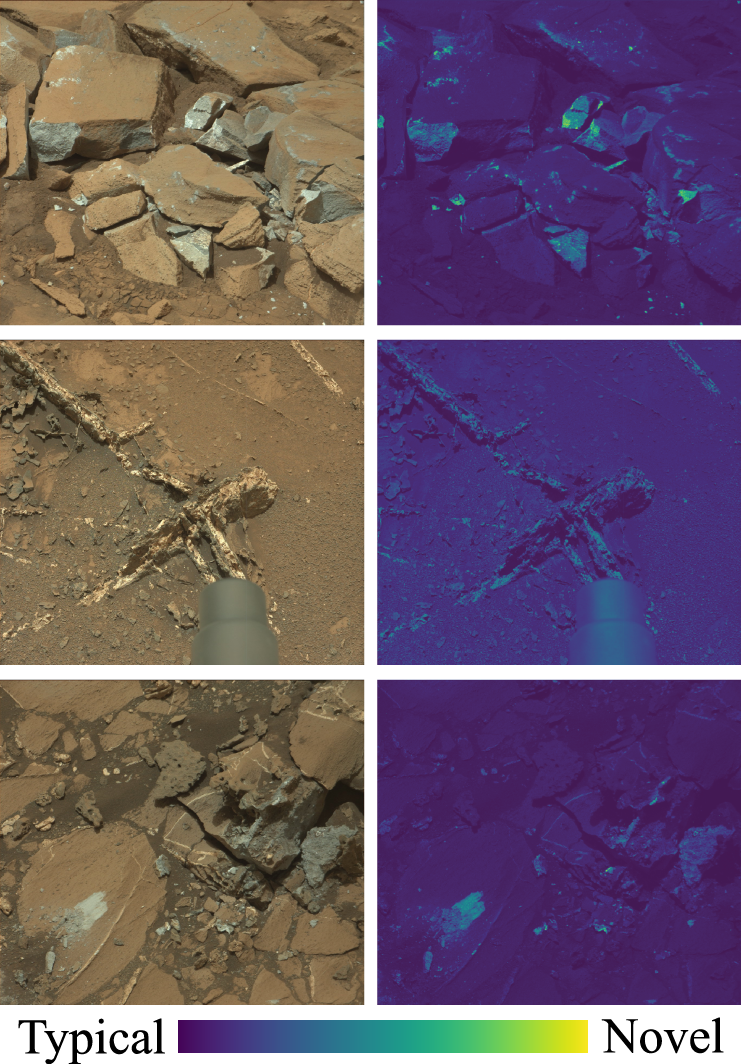
\includegraphics[width=3.25in]{figs/msl/easy.png}\\
\caption[Examples of Highlighting Novelties with RX for Mastcam Multispectral Images]{Examples of pixel novelty scores using RX for easy-to-spot novelties. The left column shows the RGB image from the sequence, and the right column shows the output from RX with a color bar ranging from typical to novel. From top to bottom: \mbox{Broken Rock (mcam05168)}, \mbox{Veins (mcam04817)}, \mbox{Dump Pile (mcam04892)}}
\label{msl/fig:easyNovel}
\end{figure}

To assist tactical operations planning, the novelty detection system is most useful when it is able to highlight features of interest that are not otherwise easily identifiable. 
Figure \ref{msl/fig:mcam12276} shows an example of such a sequence.
In this sequence, there is a ring of novel material around one of the rocks near the top of the thumbnail. 
This ring is almost unidentifiable in the RGB image and faint in filters L5 and L6. 
This ring is suspected by science team members to be due to a thin layer of brighter regolith deposited around the edge of the rock and not part of the rock composition.
By taking every filter into account, RX is able to identify the spectral anomaly around this rock and provide guidance for follow-up analysis.

\begin{figure*}
\centering
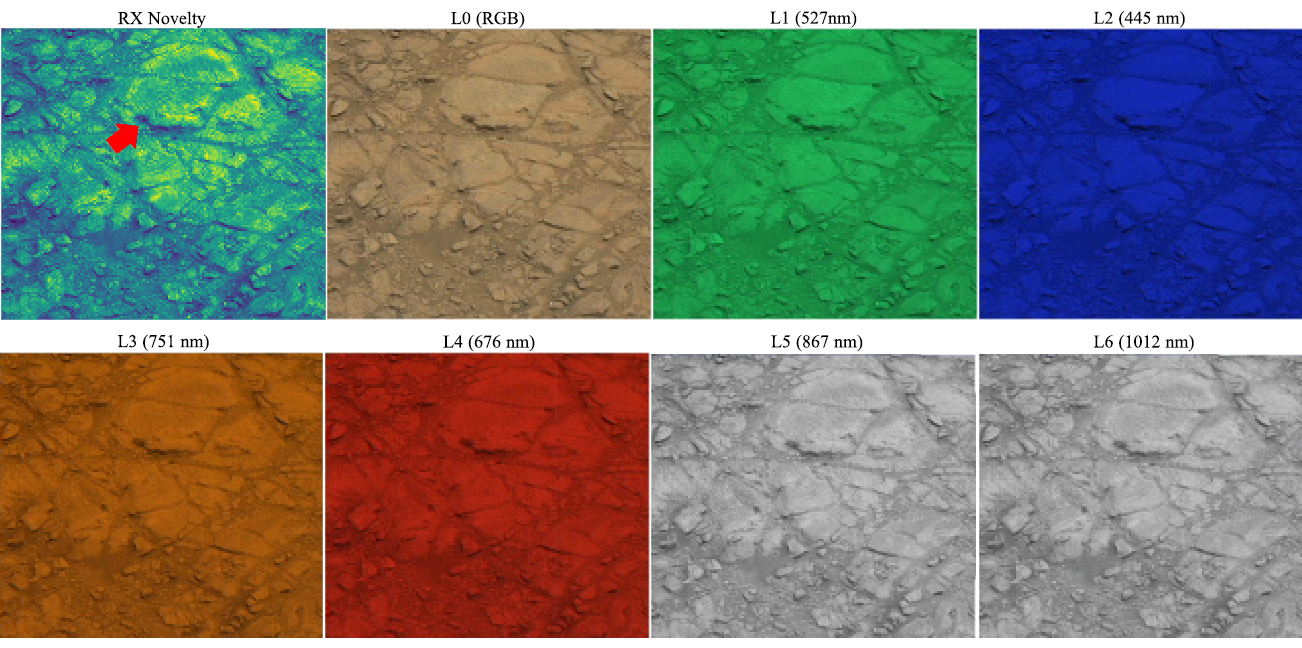
\includegraphics[width=\linewidth]{figs/msl/mcam_novel.png}
\caption[An Example of a Difficult-to-Spot Region in a Mastcam Multispectral Image, Clearly Visible in RX]{An example of difficult-to-notice novel features from mcam12276. In this example, there is a subtle ring of brighter dust on the edge of one of the rocks (shown by the red arrow). This is not noticeable in L0 (RGB) and faint in L5 (867 nm) and L6 (1012nm).}
\label{msl/fig:mcam12276}
\end{figure*}

In order to assess which sequences to analyze first, statistics about the pixel novelty scores can be calculated to rank multispectral sequences. 
Sorting by the mean pixel novelty score in each sequence orders the sequences based on mean novelty across the image.
%While the most novel sequences will rise to the top of the stack, ordering by mean pixel novelty score provides unexpected results. 
However, sorting by the mean score of all pixels in the sequence does not effectively prioritize images with obvious or localized novel features because the mean score can suppress high scores in small, localized features that are the only novel features in the image. 
%Sequences with a high average novelty score typically consist of images without any obvious novelties as the whole image has a high average score. 
In contrast, images with high mean scores that have uniformly high scores across the entire image will not show contrast in the heat map visualization and will be difficult to interpret using this visualization. 
%This type of sorting is not fitting for tactical operations analysis as the heat map provides little useful information. 
To prioritize high novelty scores corresponding to localized features, we used the maximum pixel novelty score instead to sort novel sequences, as it is better at prioritizing images with high novelty features. 
%Maximum pixel novelty score highlights sequences with clear outliers making them clearer candidates for follow up analysis. 
Examples of the top and bottom ten images sorted by maximum RX score are shown in Figure \ref{msl/fig:sorted}. 
The top-scoring sequences show images of high variability when compared with the low-scoring images. 
The highest-scoring pixels in these sequences are typically rover parts, which, while being spectrally novel, are not necessarily useful for operations.
Additionally, sequences containing shadows that move over time tend to have higher scores, as the shadow fans across the different channels and creates a rainbow.
The low-scoring sequences mostly consist of sky and sand images, which are of relatively low interest from a tactical perspective. 
When comparing multiple images, we normalized the pixel novelty scores across the data set in order to display relative novelty. 
The scores are visualized without normalization when an analyst selects an individual sequence to analyze. 

\begin{figure*}
\centering
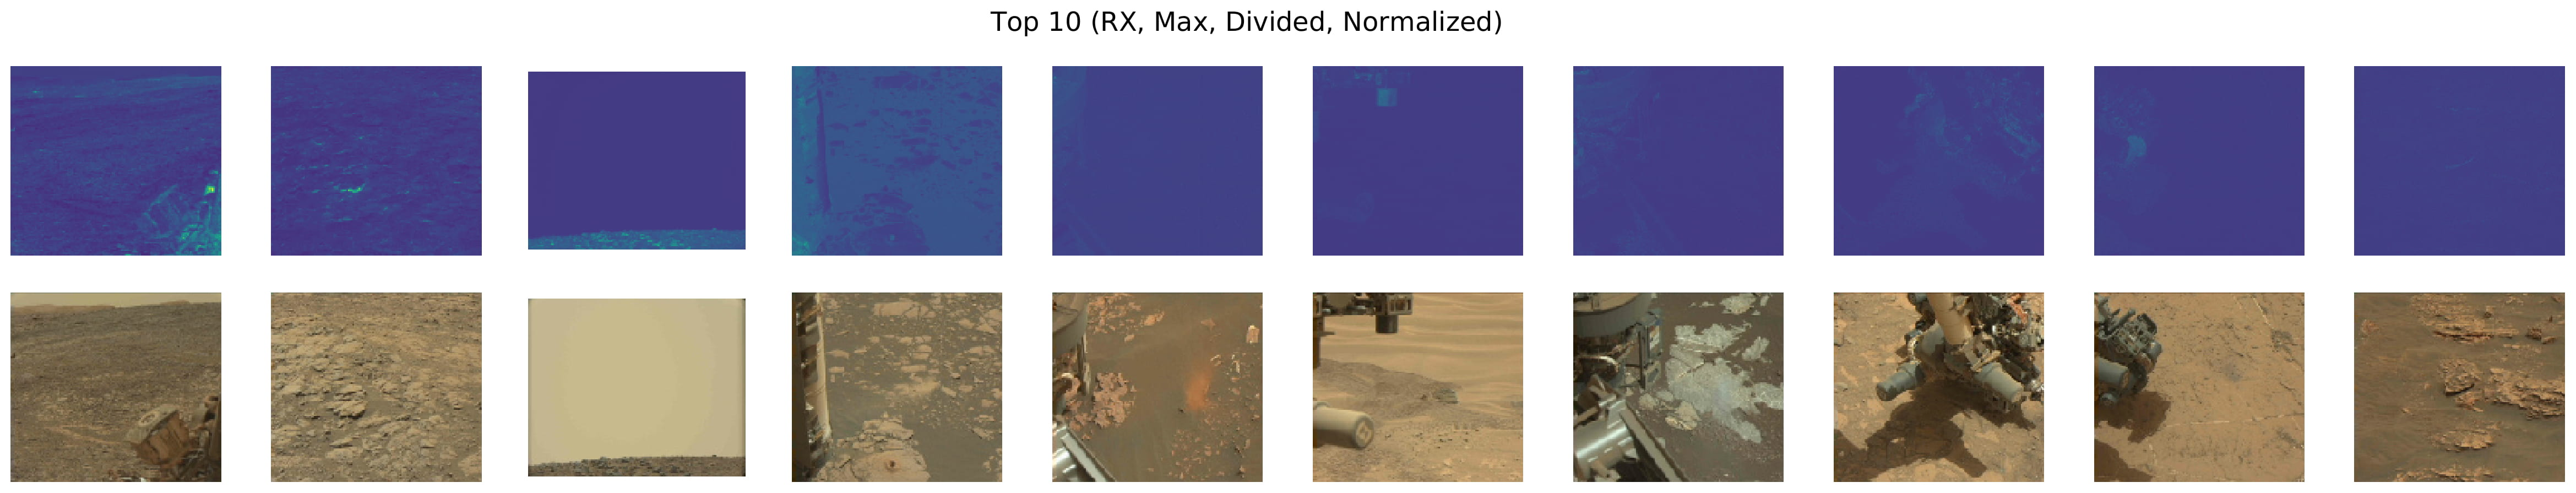
\includegraphics[width=\linewidth]{figs/msl/top10.jpg}
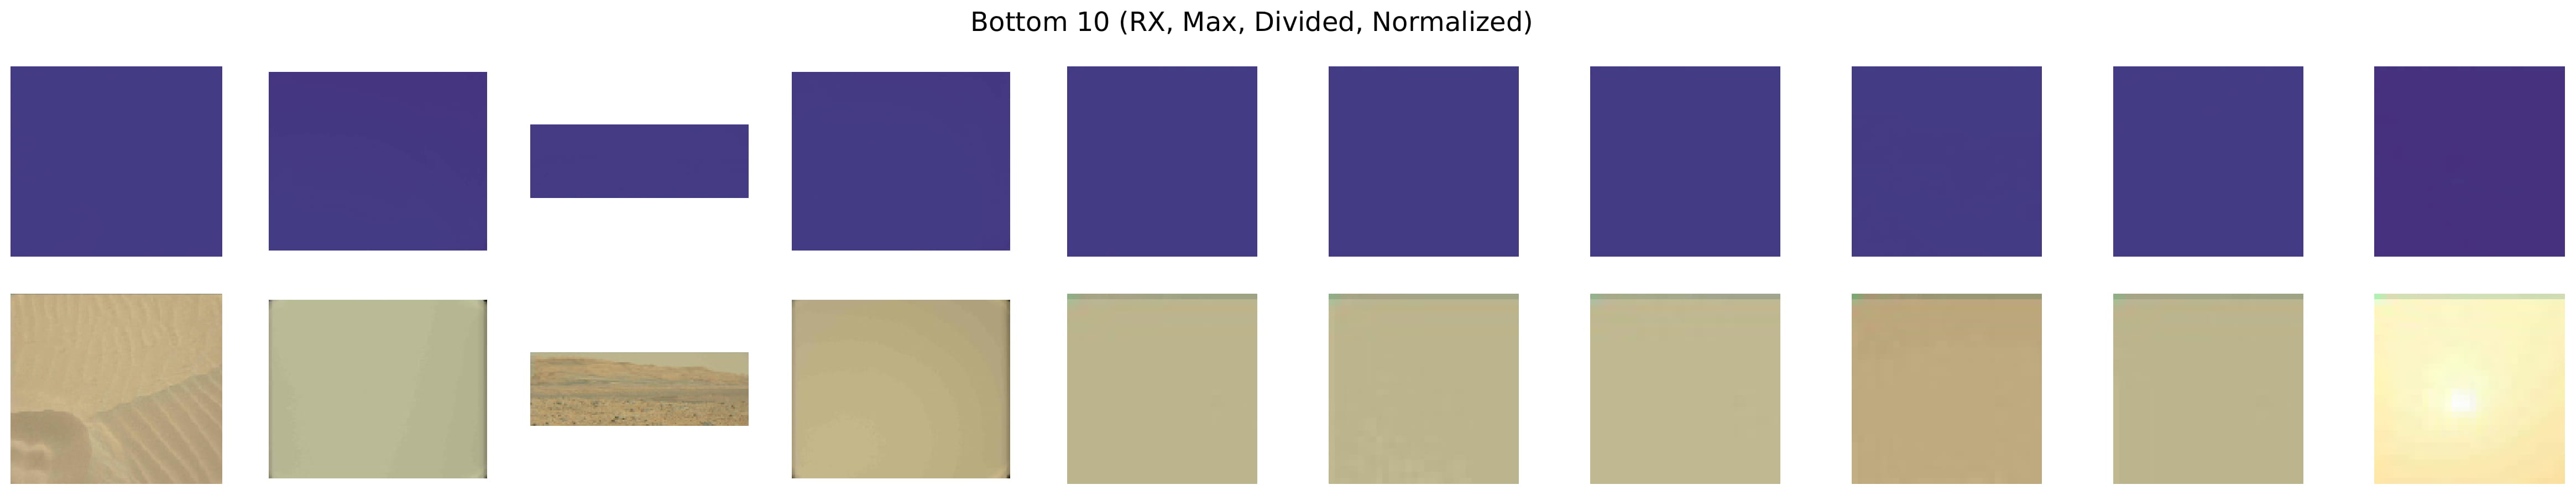
\includegraphics[width=\linewidth]{figs/msl/bottom10.jpg}
\caption[Examples of the Most and Least Novel Images in the Mastcam Left Eye Data Set]{The most and least novel sequences in the Mastcam Left Eye data set. Sequences are sorted by maximum novelty value obtained from a brightness-corrected background distribution. The pixel novelty scores are normalized across the entire data set.}
\label{msl/fig:sorted}
\end{figure*}

%%%%%%%%%%%%%%%%%%%%%%%%%%%%%%%%%%%%%%
\section{Conclusions}
%%%%%%%%%%%%%%%%%%%%%%%%%%%%%%%%%%%%%%
While initial results from reviewing the novelty detection output seem promising, it is difficult to evaluate the effectiveness of the system at assisting in operations without a longer-term study in which many sequences would be analyzed for previously undiscovered features.
This is necessary as generating a test set of undiscovered novelties is not feasible due to the fact that they haven't been discovered yet.
%tell the percentage of new novelties present. 
%As this study is looking for hard to detect novelties, generating a labeled test set for the undiscovered is not feasible.
The purpose of this study is to assist tactical planning, so the key value is in the system's ability to highlight unique sequences and novel features within those sequences. 
The brightly colored heat map of novel regions for each sequence appears to provide a fast way of identifying spots for follow-up analysis. 
The next step for this work is to gather more feedback from the tactical planning team to determine the increase in productivity while using novelty detection products.
To quantitatively evaluate this, operations staff members can be given the task of analyzing the Mastcam sequence with and without novelty-based products.
Analysis time can be recorded to identify if staff members are able to identify novel features quicker when the novelty detection system is used for triaging.
Instances, where the system highlights something that the staff member does not find novel, can also help to understand the limitations of the method and improve future method development.
This feedback will help validate the usability of the novelty detection system and fine-tune its features, such as dividing by brightness, global normalization, and limiting the training set to recent data. 
Additionally, novelty detection products may improve masking rover parts and finding ways to reduce the rainbowing effect from shadows.
Another approach may be to not use a background distribution based on the entire Mastcam multispectral history and, instead, calculate new models for each image to find the most novel feature on a local scale.

Future work is also needed to improve ways of ordering the sequences based on their novelty scores.
While sorting sequences by the maximum pixel RX score provides more useful outputs than sorting by the mean pixel RX score, there may be better ways of prioritizing sequences (e.g., sorting by the variance of scores in the image). %heat map may help to identify sequences with spectral novelties.
To validate that the ranking's priorities align with the triage an operations staff member may perform, an experiment can also be created to have both humans and the novelty detection system generate rankings.
The rankings can be compared using Spearman's rank correlation coefficient to compare their overlap.
Such an experiment could also help to find better ways of sorting the sequences.
Finding better ways to prioritize novel sequences is also beneficial for on-board autonomy applications \cite{wagstaffnovelty}.

MSLWEB, an Arizona State University-based Mastcam tracking application, is the perfect platform for integrating novelty detection products into tactical planning workflows. 
Currently, MSLWEB supports the automatic generation of simple, quick-look products such as decorrelation stretches and filter ratios. 
Augmenting this system to support novelty detection would involve adding an inference endpoint to the pipeline and automatically passing new sequences through it. 
As this system is currently being used by operations staff, a strong justification is necessary to perform this integration. 
At the time, the novelty detection system has shown promising examples of novelty highlighting and sorting. 
Further analysis is needed to demonstrate how these examples would fit into the tactical planning pipeline and the time-saving benefits they might provide.

In addition to operations, the development of the novelty and discovery API endpoints are key to enabling more intelligent ways of navigating planetary data on the PDS Image Atlas. 
Currently, both tools have running prototype endpoints available for PDS devs to begin integration with future PDS Image Atlas releases.
With the integration of these tools, the capabilities of the Image Atlas can expand to provide an overview of highly diverse images for each NASA mission, group images by similarity, and sort albums by their most interesting content.

Future work involves creating models for more instruments, implementing new algorithms, and developing user interface prototypes. 
A pipeline to deploy new endpoints has been set up on SM so that models can be developed for new instrument data sets. 
This is done by simply specifying the data location and how it should be loaded and running the pipeline on the image set. 
For novelty detection, new algorithms, such as principal component analysis and generative adversarial networks, can be adapted to the SM suite so that Image Atlas developers have more control over how they would like to sort the data. 
Finally, proper prototypes for how these tools will work with the Image Atlas need to be developed so full integration can begin.